\documentclass[10pt]{article}

% Idioma y codificación
\usepackage[utf8]{inputenc}
\usepackage[spanish]{babel}

% Márgenes
\usepackage{geometry}
\geometry{top=2.5cm, bottom=2.5cm, left=2.5cm, right=2.5cm}

% Gráficos
\usepackage{graphicx}
\usepackage{graphics}
\usepackage{wrapfig}
\usepackage{float}

% Listings para código
\usepackage{listings}
\usepackage{xcolor}
\usepackage{caption}
\usepackage{capt-of}
\lstdefinestyle{terminal}{
	backgroundcolor=\color{gray!10},
	basicstyle=\ttfamily\small,
	keywordstyle=\color{blue},
	commentstyle=\color{gray},
	frame=single,
	columns=fullflexible,
	morecomment=[l]{//}
}
\usepackage{listings}
\lstset{
	inputencoding=utf8,
	extendedchars=true,
	literate={á}{{\'a}}1 {é}{{\'e}}1 {í}{{\'i}}1 {ó}{{\'o}}1 {ú}{{\'u}}1 {ñ}{{\~n}}1
}

% Hipervínculos
\usepackage[hidelinks]{hyperref}
\hypersetup{
	colorlinks=true,
	linkcolor=blue,
	filecolor=magenta,
	urlcolor=cyan,
}

\usepackage{url}

% Encabezados y pies de página
\usepackage{fancyhdr}
\pagestyle{fancy}
\fancyhf{}
\fancyfoot[R]{\thepage}

% Formato de títulos
\usepackage{titlesec}
\titleformat{\subsection}{\normalfont\large\bfseries}{\hspace{1em}\thesubsection}{1em}{}
\titleformat{\subsubsection}{\normalfont\normalsize\bfseries}{\hspace{2em}\thesubsubsection}{1em}{}

% Datos de la portada
\title{\textbf{Cuaderno de bitácora}}
\author{\textbf{\small Daniel Sanabria Salamanqués}}
\date{\today}

\makeatletter
\let\thetitle\@title
\let\theauthor\@author
\let\thedate\@date
\makeatother

\begin{document}
	
	\begin{titlepage}
		\centering
		\includegraphics[scale=0.3]{uva-3881270087.pdf}\\[0.5cm]
		\rule{\linewidth}{0.2mm}\\[0.4cm]
		{\huge\bfseries \thetitle}\\
		\rule{\linewidth}{0.2mm}\\[1.5cm]
		{\Large\bfseries Ingeniería Informática}\\[0.3cm]
		{\Large\bfseries Tecnologías de la Información}\\[1cm]
		{\Large \theauthor}\\[1.5cm]
		{\Large \thedate}
	\end{titlepage}
	
	\renewcommand{\contentsname}{Índice}
	\tableofcontents
	\clearpage
	\section{Instalación}
	\subsection{Clúster de Máquinas Virtuales}
	Para comenzar con la instalación, me dirijo a la página \url{matrix.inf.uva.es} e inicio sesión con mi cuenta de laboratorio de la escuela. Una vez hecho, observo que en el \verb|Datacenter| se encuentra mi máquina virtual \verb|vm3803.virtual.lab.inf.uva.es|. Al hacer doble clic, compruebo en la sección de \verb|Hardware| si está en el apartado \verb|CD/DVD| la imagen de \verb|Ubuntu Server|. Como no aparece, hago clic sobre ese apartado y con la opción \verb|Edit| que aparece en la parte superior, agrego la imagen a ese disco de la máquina.
	\subsection{Configuración de instalación}
	Tras esto, voy a la sección \verb|Console| para iniciar la máquina virtual y comenzar con la instalación de \verb|Ubuntu Server|. Lo primero es seleccionar el idioma para el sistema; en mi caso, escojo inglés. Después, indico que no quiero realizar la actualización para obtener \verb|Ubuntu Server 25.04|. Luego, para la configuración del teclado, selecciono el teclado español, debido a que mi teclado necesita esa configuración. En la siguiente pantalla, escojo que la instalación base será \verb|Ubuntu Server| por defecto y sin opciones adicionales. En la configuración de red, no modifico ningún valor ni agrego ningún \verb|proxy|. En cuanto al almacenamiento, indico que para la instalación use todo el disco y que no lo monte como un grupo \verb|LVM|. Después de confirmar la configuración del almacenamiento, relleno en la siguiente pantalla los datos de mi perfil:
	\begin{itemize}
		\item \textbf{Nombre}: Daniel
		\item \textbf{Nombre de servidor}: vm3803
		\item \textbf{Username}: dansana
	\end{itemize}
	Para la configuración de la conexión SSH, selecciono la opción de que se instale \verb|OpenSSH|. Para terminar, no agrego ninguna \verb|snap| al sistema y después de seleccionar \verb|Done|, dejo que se termine la instalación con la configuración seleccionada. Tras unos minutos, la instalación termina y reinicio el sistema.\\\\
	Una vez que ha arrancado, inicio sesión con el usuario y la contraseña que he creado y, acto seguido, procedo a purgar ciertas aplicaciones que no son necesarias.
	\subsection{Reconocimiento del entorno}
	Nos piden realizar un reconocimiento del entorno para conocer acerca del sistema que hemos instalado, además de saber cómo funciona la máquina virtual en la página \url{matrix.inf.uva.es}:
	\begin{itemize}
		\item \textbf{Version Kernel Linux}: El comando \verb|cat /proc/version|, nos devuelve la información acerca del Linux instalado. En este caso, se trata de un Linux con la versión el kernel 6.8.0-79-generic. El funcionamiento del comando es mostrar lo que contiene el archivo \verb|version| dentro de \verb|proc|, que se trata del sistema de ficheros.
		\item \textbf{Particiones}: Con el comando \verb|df -h|, se obtiene las particiones montadas. En este caso, tenemos las siguientes particiones:
		\begin{itemize}
			\item \textit{/dev/sda1}: Montada en el directorio \verb|/boot/efi| y es la encargada de el arranque del sistema. 
			\item \textit{/dev/sda2}: Montada en el directorio raíz \verb|/|, dedicada al resto de sistema.
		\end{itemize}
		\item \textbf{Espacio libre}: Con el mismo comando que el punto anterior, se puede ver que hay varias columnas dedicadas al almacenamiento de cada partición:
		\begin{itemize}
			\item \textit{/dev/sda1}: Con \verb|1.1G| en total, solo se ha usado el 1\%, es decir, \verb|6.2M| se ha utilizado y se encuentran disponibles \verb|1.1G| para usar.
			\item \textit{/dev/sda2}: Con \verb|58G| en total, solo se ha usado el 12\%, es decir, \verb|6.5G| se ha utilizado y se encuentran disponibles \verb|49G| para usar.
		\end{itemize}
		\item \textbf{Cerrar sesión}: Cuando se ha iniciado sesión y queremos cerrar esa misma sesión, simplemente tenemos que escribir el comando \verb|logout| y el sistema cerrará la sesión.
		\item \textbf{Apagar la máquina}: Desde la consola del sistema, mediante el comando \verb|shutdown -h| se le enviará una señal al sistema para apagar la máquina.
		\item \textbf{Reiniciar la máquina}: Para el reinicio, se emplea el comando \verb|reboot|.
		\item \textbf{Controles de la consola de la máquina virtual}: Se pide usar los controles que aparecen en la parte superior:
		\begin{enumerate}
			\item Cuando la máquina esté encendida, nos indican apagar la máquina con \verb|Stop|. Esto obligará a la máquina a hacer un apagado forzado.
			\item Después de volver a encender, nos piden restear la máquina mediante la opción \verb|Reset|. Funciona igual que escribir el comando \verb|reboot|.
			\item Por último, será apagar de nuevo la máquina pero con la opción \verb|Shutdown| que será lo mismo que escribir el comando \verb|shutdown -h|.
		\end{enumerate}
	\end{itemize}
	\subsection{Acceso remoto vía ssh}
	Se nos indica que el sistema ya tiene instalado y activado el servicio de conexión segura \verb|sshd| (que previamente hemos configurado en la configuración de la instalación) y para comprobar que funciona correctamente, me conectaré desde \verb|Jair| a esta máquina, usando la red de la UVa. Aquí se muestra una captura del proceso:
	\begin{figure}[H]
		\setlength{\abovecaptionskip}{0cm}
		\setlength{\belowcaptionskip}{0cm}
		\centering
		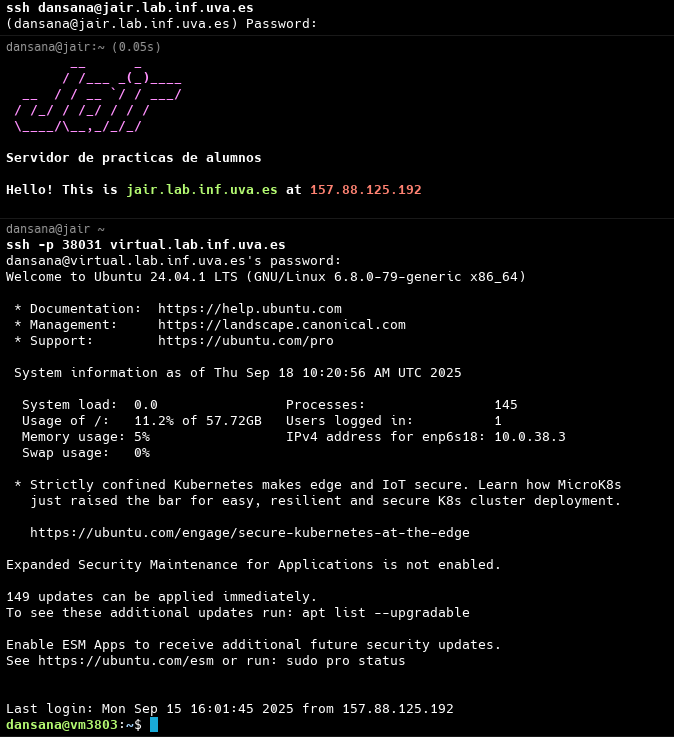
\includegraphics[width=0.6\linewidth]{Recursos/ssh.png}
		\label{fig:datos}
	\end{figure}
	\subsection{Activar cuenta root}
	Lo siguiente que se indica es activar la cuenta \verb|root| cambiando su contraseña mediante \verb|sudo passwd root| e indicando una clave para ese usuario y así poder acceder a la consola directamente como \verb|root|, ya que por defecto no trae ninguna contraseña y puede ser una brecha de seguridad.
	\subsection{Trabajo No Presencial}
	\begin{itemize}
		\item \textbf{Administración de discos – particiones}: 
		\begin{itemize}
			\item Los discos duros o dispositivos de bloques, se dividen en unidades lógicas llamadas \textit{particiones}.\cite{Discos}
			\item Una partición sirven organizan y almacenan el sistema operativo, las aplicaciones y los archivos personales. Existen diferentes esquemas de particiones para la distribución de particiones en un disco, como MBR o GPT.
			\item Cada partición se representa como un archivo en el sistema de archivos de Linux y se encuentra ubicada en el directorio \verb|/dev|.
		\end{itemize}
		\item \textbf{Sistemas de archivos}: 
		\begin{itemize}
			\item Se organizan en una estructura jerárquica, de tipo árbol. El nivel más alto del sistema de ficheros es / o directorio raíz. Todos los demás ficheros y directorios están bajo el directorio raíz.\cite{Archivos}
			\item Por debajo del directorio raíz (/) hay un importante grupo de directorios común a la mayoría de las distribuciones de GNU/Linux: \verb|/bin, /boot, /etc/, /opt, etc|.
		\end{itemize}
		\item \textbf{Actualización de un sistema operativo previamente instalado}:
		\begin{itemize}
			\item En el caso de nuestra máquina virtual, estamos trabajando con \verb|Ubuntu| que pertenece al grupo de distribuciones \verb|Debian|, por lo que para actualizar el sistema operativo una vez instalado se hará uso de la herramienta \verb|apt|.
			\item \verb|apt| nos proporciona un sistema de gestión de paquetes donde maneja automáticamente las dependencias para la instalación de esos paquetes. Requiere de privilegios administrativos.\cite{Actualizar}
			\item Para las actualizaciones será necesario usar los comandos \verb|sudo apt update| y \verb|sudo apt upgrade|.
		\end{itemize}
		\item \textbf{Identificación discos duros}:
		\item \textbf{Sistema de ficheros}:
		\item \textbf{RAID}:
	\end{itemize}
	
	\clearpage
	\bibliographystyle{plain}
	\bibliography{bibliografia}
\end{document}